\documentclass{standalone}
\usepackage{tikz}
\usetikzlibrary{patterns, positioning}


\begin{document}
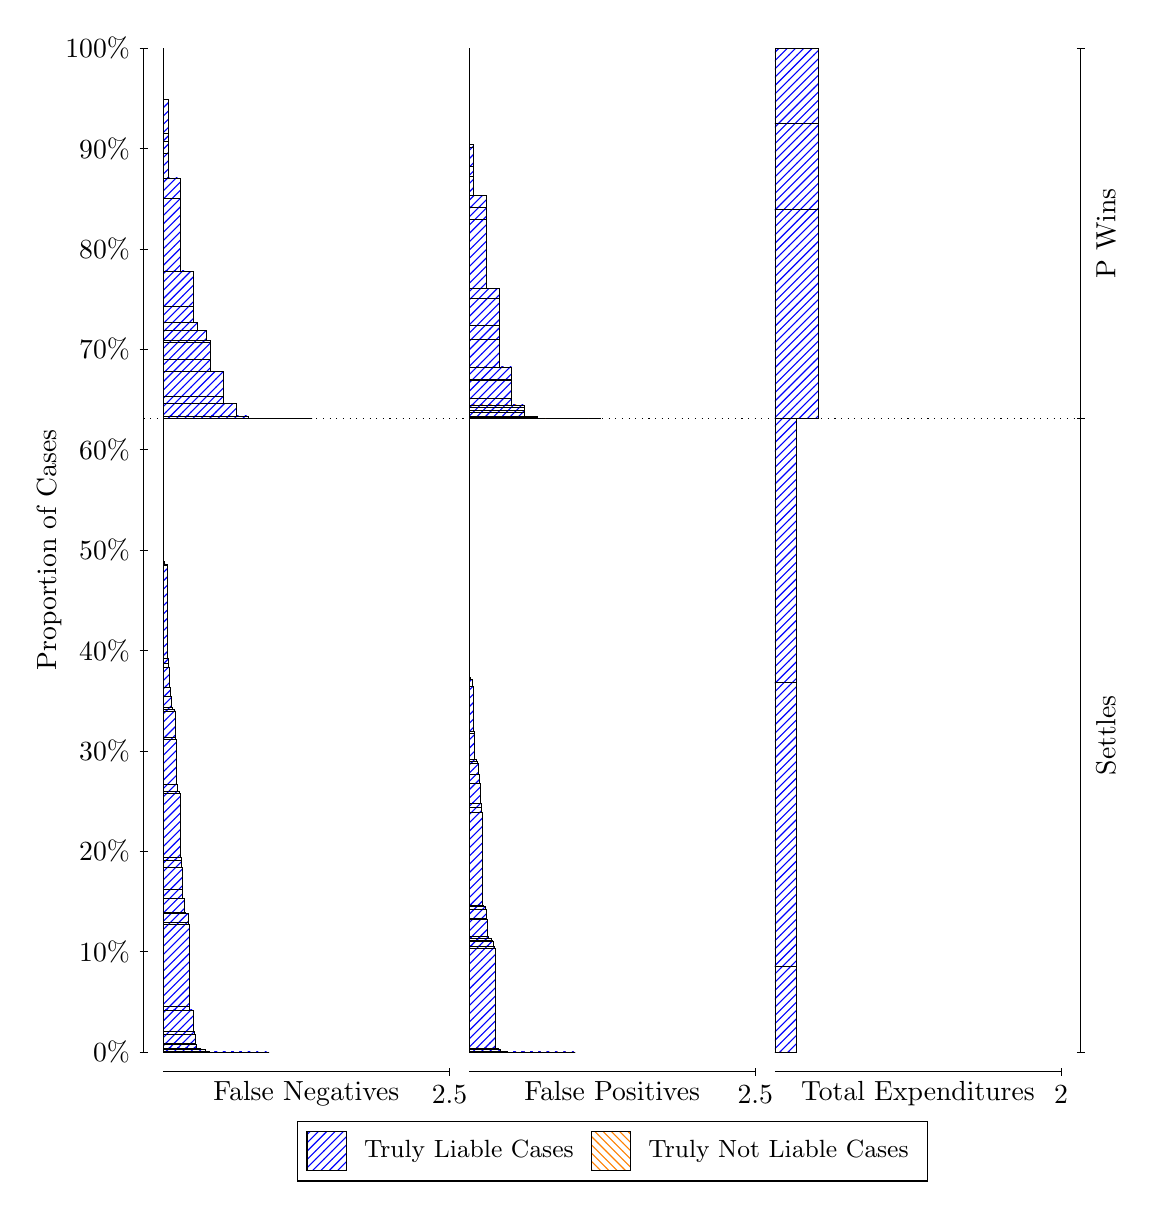
\begin{tikzpicture}
\draw[black, very thin] (1.5,1.75) -- (1.5,14.5);
\node[rotate=90, text=black, anchor=center] at (0.3, 8.125) {Proportion of Cases};
\draw[black, very thin] (1.45,1.75) -- (1.55,1.75);
\node[text=black, anchor=east] at (1.45, 1.75) {0\%};
\draw[black, very thin] (1.45,3.025) -- (1.55,3.025);
\node[text=black, anchor=east] at (1.45, 3.025) {10\%};
\draw[black, very thin] (1.45,4.3) -- (1.55,4.3);
\node[text=black, anchor=east] at (1.45, 4.3) {20\%};
\draw[black, very thin] (1.45,5.575) -- (1.55,5.575);
\node[text=black, anchor=east] at (1.45, 5.575) {30\%};
\draw[black, very thin] (1.45,6.85) -- (1.55,6.85);
\node[text=black, anchor=east] at (1.45, 6.85) {40\%};
\draw[black, very thin] (1.45,8.125) -- (1.55,8.125);
\node[text=black, anchor=east] at (1.45, 8.125) {50\%};
\draw[black, very thin] (1.45,9.4) -- (1.55,9.4);
\node[text=black, anchor=east] at (1.45, 9.4) {60\%};
\draw[black, very thin] (1.45,10.675) -- (1.55,10.675);
\node[text=black, anchor=east] at (1.45, 10.675) {70\%};
\draw[black, very thin] (1.45,11.95) -- (1.55,11.95);
\node[text=black, anchor=east] at (1.45, 11.95) {80\%};
\draw[black, very thin] (1.45,13.225) -- (1.55,13.225);
\node[text=black, anchor=east] at (1.45, 13.225) {90\%};
\draw[black, very thin] (1.45,14.5) -- (1.55,14.5);
\node[text=black, anchor=east] at (1.45, 14.5) {100\%};

\draw[black, very thin] (13.4,1.75) -- (13.4,14.5);
\draw[black, very thin] (13.35,1.75) -- (13.45,1.75);
\node[anchor=west] at (13.35, 1.75) {};
\draw[black, very thin] (13.35,9.7946) -- (13.45,9.7946);
\node[anchor=west] at (13.35, 9.7946) {};
\draw[black, very thin] (13.35,14.5) -- (13.45,14.5);
\node[anchor=west] at (13.35, 14.5) {};

\draw[black, very thin, pattern color=blue, pattern=north east lines] (1.75,1.75) rectangle (3.0943,1.75);
\draw[black, very thin, pattern color=blue, pattern=north east lines] (1.75,1.75) rectangle (2.949,1.75);
\draw[black, very thin, pattern color=blue, pattern=north east lines] (1.75,1.75) rectangle (2.9329,1.75);
\draw[black, very thin, pattern color=blue, pattern=north east lines] (1.75,1.75) rectangle (2.8763,1.75);
\draw[black, very thin, pattern color=blue, pattern=north east lines] (1.75,1.75) rectangle (2.8037,1.75);
\draw[black, very thin, pattern color=blue, pattern=north east lines] (1.75,1.75) rectangle (2.7875,1.75);
\draw[black, very thin, pattern color=blue, pattern=north east lines] (1.75,1.75) rectangle (2.7714,1.75);
\draw[black, very thin, pattern color=blue, pattern=north east lines] (1.75,1.75) rectangle (2.731,1.75);
\draw[black, very thin, pattern color=blue, pattern=north east lines] (1.75,1.75) rectangle (2.7149,1.75);
\draw[black, very thin, pattern color=blue, pattern=north east lines] (1.75,1.75) rectangle (2.6583,1.75);
\draw[black, very thin, pattern color=blue, pattern=north east lines] (1.75,1.75) rectangle (2.6422,1.75);
\draw[black, very thin, pattern color=blue, pattern=north east lines] (1.75,1.75) rectangle (2.626,1.75);
\draw[black, very thin, pattern color=blue, pattern=north east lines] (1.75,1.75) rectangle (2.6099,1.75);
\draw[black, very thin, pattern color=blue, pattern=north east lines] (1.75,1.75) rectangle (2.5857,1.75);
\draw[black, very thin, pattern color=blue, pattern=north east lines] (1.75,1.75) rectangle (2.5695,1.75);
\draw[black, very thin, pattern color=blue, pattern=north east lines] (1.75,1.75) rectangle (2.5534,1.75);
\draw[black, very thin, pattern color=blue, pattern=north east lines] (1.75,1.75) rectangle (2.513,1.75);
\draw[black, very thin, pattern color=blue, pattern=north east lines] (1.75,1.75) rectangle (2.4969,1.75);
\draw[black, very thin, pattern color=blue, pattern=north east lines] (1.75,1.75) rectangle (2.4807,1.75);
\draw[black, very thin, pattern color=blue, pattern=north east lines] (1.75,1.75) rectangle (2.4646,1.75);
\draw[black, very thin, pattern color=blue, pattern=north east lines] (1.75,1.75) rectangle (2.4484,1.7506);
\draw[black, very thin, pattern color=blue, pattern=north east lines] (1.75,1.7506) rectangle (2.4403,1.7506);
\draw[black, very thin, pattern color=blue, pattern=north east lines] (1.75,1.7506) rectangle (2.4242,1.7506);
\draw[black, very thin, pattern color=blue, pattern=north east lines] (1.75,1.7506) rectangle (2.408,1.7506);
\draw[black, very thin, pattern color=blue, pattern=north east lines] (1.75,1.7506) rectangle (2.3919,1.7508);
\draw[black, very thin, pattern color=blue, pattern=north east lines] (1.75,1.7508) rectangle (2.3677,1.7508);
\draw[black, very thin, pattern color=blue, pattern=north east lines] (1.75,1.7508) rectangle (2.3515,1.7508);
\draw[black, very thin, pattern color=blue, pattern=north east lines] (1.75,1.7508) rectangle (2.3354,1.7528);
\draw[black, very thin, pattern color=blue, pattern=north east lines] (1.75,1.7528) rectangle (2.3192,1.7533);
\draw[black, very thin, pattern color=blue, pattern=north east lines] (1.75,1.7533) rectangle (2.3031,1.7552);
\draw[black, very thin, pattern color=blue, pattern=north east lines] (1.75,1.7552) rectangle (2.295,1.7552);
\draw[black, very thin, pattern color=blue, pattern=north east lines] (1.75,1.7552) rectangle (2.2869,1.7815);
\draw[black, very thin, pattern color=blue, pattern=north east lines] (1.75,1.7815) rectangle (2.2789,1.7816);
\draw[black, very thin, pattern color=blue, pattern=north east lines] (1.75,1.7816) rectangle (2.2627,1.7816);
\draw[black, very thin, pattern color=blue, pattern=north east lines] (1.75,1.7816) rectangle (2.2466,1.7859);
\draw[black, very thin, pattern color=blue, pattern=north east lines] (1.75,1.7859) rectangle (2.2304,1.7905);
\draw[black, very thin, pattern color=blue, pattern=north east lines] (1.75,1.7905) rectangle (2.2223,1.8016);
\draw[black, very thin, pattern color=blue, pattern=north east lines] (1.75,1.8016) rectangle (2.2062,1.8019);
\draw[black, very thin, pattern color=blue, pattern=north east lines] (1.75,1.8019) rectangle (2.19,1.8023);
\draw[black, very thin, pattern color=blue, pattern=north east lines] (1.75,1.8023) rectangle (2.1739,1.8453);
\draw[black, very thin, pattern color=blue, pattern=north east lines] (1.75,1.8453) rectangle (2.1577,1.864);
\draw[black, very thin, pattern color=blue, pattern=north east lines] (1.75,1.864) rectangle (2.1497,1.9749);
\draw[black, very thin, pattern color=blue, pattern=north east lines] (1.75,1.9749) rectangle (2.1416,2.0076);
\draw[black, very thin, pattern color=blue, pattern=north east lines] (1.75,2.0076) rectangle (2.1335,2.0095);
\draw[black, very thin, pattern color=blue, pattern=north east lines] (1.75,2.0095) rectangle (2.1254,2.2813);
\draw[black, very thin, pattern color=blue, pattern=north east lines] (1.75,2.2813) rectangle (2.1174,2.2844);
\draw[black, very thin, pattern color=blue, pattern=north east lines] (1.75,2.2844) rectangle (2.1012,2.2849);
\draw[black, very thin, pattern color=blue, pattern=north east lines] (1.75,2.2849) rectangle (2.0851,2.3301);
\draw[black, very thin, pattern color=blue, pattern=north east lines] (1.75,2.3301) rectangle (2.077,3.3707);
\draw[black, very thin, pattern color=blue, pattern=north east lines] (1.75,3.3707) rectangle (2.0689,3.3955);
\draw[black, very thin, pattern color=blue, pattern=north east lines] (1.75,3.3955) rectangle (2.0609,3.5077);
\draw[black, very thin, pattern color=blue, pattern=north east lines] (1.75,3.5077) rectangle (2.0447,3.5131);
\draw[black, very thin, pattern color=blue, pattern=north east lines] (1.75,3.5131) rectangle (2.0286,3.5203);
\draw[black, very thin, pattern color=blue, pattern=north east lines] (1.75,3.5203) rectangle (2.0124,3.6998);
\draw[black, very thin, pattern color=blue, pattern=north east lines] (1.75,3.6998) rectangle (1.9963,3.8178);
\draw[black, very thin, pattern color=blue, pattern=north east lines] (1.75,3.8178) rectangle (1.9882,4.0948);
\draw[black, very thin, pattern color=blue, pattern=north east lines] (1.75,4.0948) rectangle (1.9801,4.1899);
\draw[black, very thin, pattern color=blue, pattern=north east lines] (1.75,4.1899) rectangle (1.972,4.2171);
\draw[black, very thin, pattern color=blue, pattern=north east lines] (1.75,4.2171) rectangle (1.964,5.0371);
\draw[black, very thin, pattern color=blue, pattern=north east lines] (1.75,5.0371) rectangle (1.9559,5.0563);
\draw[black, very thin, pattern color=blue, pattern=north east lines] (1.75,5.0563) rectangle (1.9397,5.0598);
\draw[black, very thin, pattern color=blue, pattern=north east lines] (1.75,5.0598) rectangle (1.9236,5.1505);
\draw[black, very thin, pattern color=blue, pattern=north east lines] (1.75,5.1505) rectangle (1.9155,5.7218);
\draw[black, very thin, pattern color=blue, pattern=north east lines] (1.75,5.7218) rectangle (1.9074,5.7475);
\draw[black, very thin, pattern color=blue, pattern=north east lines] (1.75,5.7475) rectangle (1.8994,6.0806);
\draw[black, very thin, pattern color=blue, pattern=north east lines] (1.75,6.0806) rectangle (1.8832,6.1051);
\draw[black, very thin, pattern color=blue, pattern=north east lines] (1.75,6.1051) rectangle (1.8671,6.1232);
\draw[black, very thin, pattern color=blue, pattern=north east lines] (1.75,6.1232) rectangle (1.8509,6.266);
\draw[black, very thin, pattern color=blue, pattern=north east lines] (1.75,6.266) rectangle (1.8348,6.3841);
\draw[black, very thin, pattern color=blue, pattern=north east lines] (1.75,6.3841) rectangle (1.8267,6.6301);
\draw[black, very thin, pattern color=blue, pattern=north east lines] (1.75,6.6301) rectangle (1.8186,6.6837);
\draw[black, very thin, pattern color=blue, pattern=north east lines] (1.75,6.6837) rectangle (1.8106,6.7513);
\draw[black, very thin, pattern color=blue, pattern=north east lines] (1.75,6.7513) rectangle (1.8025,7.9271);
\draw[black, very thin, pattern color=blue, pattern=north east lines] (1.75,7.9271) rectangle (1.7944,7.9463);
\draw[black, very thin, pattern color=blue, pattern=north east lines] (1.75,7.9463) rectangle (1.7783,7.9497);
\draw[black, very thin, pattern color=blue, pattern=north east lines] (1.75,7.9497) rectangle (1.7621,7.9821);
\draw[black, very thin, pattern color=blue, pattern=north east lines] (1.75,7.9821) rectangle (1.754,8.1001);
\draw[black, very thin, pattern color=orange, pattern=north west lines] (1.75,8.1001) rectangle (1.75,8.1001);
\draw[black, very thin, pattern color=blue, pattern=north east lines] (1.75,8.1001) rectangle (1.75,9.7946);
\draw[black, very thin, pattern color=blue, pattern=north east lines] (1.75,9.7946) rectangle (3.6393,9.7946);
\draw[black, very thin, pattern color=blue, pattern=north east lines] (1.75,9.7946) rectangle (3.4779,9.7946);
\draw[black, very thin, pattern color=blue, pattern=north east lines] (1.75,9.7946) rectangle (3.3164,9.7946);
\draw[black, very thin, pattern color=blue, pattern=north east lines] (1.75,9.7946) rectangle (3.1549,9.7947);
\draw[black, very thin, pattern color=blue, pattern=north east lines] (1.75,9.7947) rectangle (3.1549,9.7948);
\draw[black, very thin, pattern color=blue, pattern=north east lines] (1.75,9.7948) rectangle (3.0984,9.7948);
\draw[black, very thin, pattern color=blue, pattern=north east lines] (1.75,9.7948) rectangle (2.9934,9.7969);
\draw[black, very thin, pattern color=blue, pattern=north east lines] (1.75,9.7969) rectangle (2.9934,9.7983);
\draw[black, very thin, pattern color=blue, pattern=north east lines] (1.75,9.7983) rectangle (2.9369,9.7983);
\draw[black, very thin, pattern color=blue, pattern=north east lines] (1.75,9.7983) rectangle (2.8319,9.8293);
\draw[black, very thin, pattern color=blue, pattern=north east lines] (1.75,9.8293) rectangle (2.7754,9.8293);
\draw[black, very thin, pattern color=blue, pattern=north east lines] (1.75,9.8293) rectangle (2.7754,9.8293);
\draw[black, very thin, pattern color=blue, pattern=north east lines] (1.75,9.8293) rectangle (2.6704,9.9884);
\draw[black, very thin, pattern color=blue, pattern=north east lines] (1.75,9.9884) rectangle (2.6139,9.9886);
\draw[black, very thin, pattern color=blue, pattern=north east lines] (1.75,9.9886) rectangle (2.509,10.08);
\draw[black, very thin, pattern color=blue, pattern=north east lines] (1.75,10.08) rectangle (2.509,10.389);
\draw[black, very thin, pattern color=blue, pattern=north east lines] (1.75,10.389) rectangle (2.4524,10.393);
\draw[black, very thin, pattern color=blue, pattern=north east lines] (1.75,10.393) rectangle (2.4524,10.397);
\draw[black, very thin, pattern color=blue, pattern=north east lines] (1.75,10.397) rectangle (2.3475,10.542);
\draw[black, very thin, pattern color=blue, pattern=north east lines] (1.75,10.542) rectangle (2.3475,10.765);
\draw[black, very thin, pattern color=blue, pattern=north east lines] (1.75,10.765) rectangle (2.3475,10.783);
\draw[black, very thin, pattern color=blue, pattern=north east lines] (1.75,10.783) rectangle (2.291,10.914);
\draw[black, very thin, pattern color=blue, pattern=north east lines] (1.75,10.914) rectangle (2.186,11.015);
\draw[black, very thin, pattern color=blue, pattern=north east lines] (1.75,11.015) rectangle (2.1295,11.218);
\draw[black, very thin, pattern color=blue, pattern=north east lines] (1.75,11.218) rectangle (2.1295,11.662);
\draw[black, very thin, pattern color=blue, pattern=north east lines] (1.75,11.662) rectangle (2.0245,11.662);
\draw[black, very thin, pattern color=blue, pattern=north east lines] (1.75,11.662) rectangle (2.0245,11.669);
\draw[black, very thin, pattern color=blue, pattern=north east lines] (1.75,11.669) rectangle (2.0245,11.669);
\draw[black, very thin, pattern color=blue, pattern=north east lines] (1.75,11.669) rectangle (1.968,12.589);
\draw[black, very thin, pattern color=blue, pattern=north east lines] (1.75,12.589) rectangle (1.968,12.851);
\draw[black, very thin, pattern color=blue, pattern=north east lines] (1.75,12.851) rectangle (1.863,12.851);
\draw[black, very thin, pattern color=blue, pattern=north east lines] (1.75,12.851) rectangle (1.863,12.851);
\draw[black, very thin, pattern color=blue, pattern=north east lines] (1.75,12.851) rectangle (1.8065,13.161);
\draw[black, very thin, pattern color=blue, pattern=north east lines] (1.75,13.161) rectangle (1.8065,13.311);
\draw[black, very thin, pattern color=blue, pattern=north east lines] (1.75,13.311) rectangle (1.8065,13.416);
\draw[black, very thin, pattern color=blue, pattern=north east lines] (1.75,13.416) rectangle (1.8065,13.844);
\draw[black, very thin, pattern color=orange, pattern=north west lines] (1.75,13.844) rectangle (1.75,13.844);
\draw[black, very thin, pattern color=blue, pattern=north east lines] (1.75,13.844) rectangle (1.75,14.5);
\draw[black, very thin, pattern color=orange, pattern=north west lines] (5.6333,1.75) rectangle (6.9777,1.75);
\draw[black, very thin, pattern color=blue, pattern=north east lines] (5.6333,1.75) rectangle (6.9777,1.75);
\draw[black, very thin, pattern color=orange, pattern=north west lines] (5.6333,1.75) rectangle (6.905,1.75);
\draw[black, very thin, pattern color=blue, pattern=north east lines] (5.6333,1.75) rectangle (6.905,1.75);
\draw[black, very thin, pattern color=orange, pattern=north west lines] (5.6333,1.75) rectangle (6.8323,1.75);
\draw[black, very thin, pattern color=blue, pattern=north east lines] (5.6333,1.75) rectangle (6.8323,1.75);
\draw[black, very thin, pattern color=blue, pattern=north east lines] (5.6333,1.75) rectangle (6.8162,1.75);
\draw[black, very thin, pattern color=orange, pattern=north west lines] (5.6333,1.75) rectangle (6.7597,1.75);
\draw[black, very thin, pattern color=blue, pattern=north east lines] (5.6333,1.75) rectangle (6.7597,1.75);
\draw[black, very thin, pattern color=blue, pattern=north east lines] (5.6333,1.75) rectangle (6.7435,1.75);
\draw[black, very thin, pattern color=orange, pattern=north west lines] (5.6333,1.75) rectangle (6.687,1.75);
\draw[black, very thin, pattern color=blue, pattern=north east lines] (5.6333,1.75) rectangle (6.687,1.75);
\draw[black, very thin, pattern color=blue, pattern=north east lines] (5.6333,1.75) rectangle (6.6709,1.75);
\draw[black, very thin, pattern color=blue, pattern=north east lines] (5.6333,1.75) rectangle (6.6547,1.75);
\draw[black, very thin, pattern color=orange, pattern=north west lines] (5.6333,1.75) rectangle (6.6143,1.75);
\draw[black, very thin, pattern color=blue, pattern=north east lines] (5.6333,1.75) rectangle (6.6143,1.75);
\draw[black, very thin, pattern color=blue, pattern=north east lines] (5.6333,1.75) rectangle (6.5982,1.75);
\draw[black, very thin, pattern color=blue, pattern=north east lines] (5.6333,1.75) rectangle (6.582,1.75);
\draw[black, very thin, pattern color=orange, pattern=north west lines] (5.6333,1.75) rectangle (6.5417,1.75);
\draw[black, very thin, pattern color=blue, pattern=north east lines] (5.6333,1.75) rectangle (6.5417,1.75);
\draw[black, very thin, pattern color=blue, pattern=north east lines] (5.6333,1.75) rectangle (6.5255,1.75);
\draw[black, very thin, pattern color=blue, pattern=north east lines] (5.6333,1.75) rectangle (6.5094,1.75);
\draw[black, very thin, pattern color=blue, pattern=north east lines] (5.6333,1.75) rectangle (6.4932,1.75);
\draw[black, very thin, pattern color=orange, pattern=north west lines] (5.6333,1.75) rectangle (6.469,1.75);
\draw[black, very thin, pattern color=blue, pattern=north east lines] (5.6333,1.75) rectangle (6.469,1.75);
\draw[black, very thin, pattern color=blue, pattern=north east lines] (5.6333,1.75) rectangle (6.4529,1.75);
\draw[black, very thin, pattern color=blue, pattern=north east lines] (5.6333,1.75) rectangle (6.4367,1.75);
\draw[black, very thin, pattern color=blue, pattern=north east lines] (5.6333,1.75) rectangle (6.4206,1.75);
\draw[black, very thin, pattern color=orange, pattern=north west lines] (5.6333,1.75) rectangle (6.3963,1.75);
\draw[black, very thin, pattern color=blue, pattern=north east lines] (5.6333,1.75) rectangle (6.3963,1.75);
\draw[black, very thin, pattern color=blue, pattern=north east lines] (5.6333,1.75) rectangle (6.3802,1.75);
\draw[black, very thin, pattern color=blue, pattern=north east lines] (5.6333,1.75) rectangle (6.364,1.75);
\draw[black, very thin, pattern color=blue, pattern=north east lines] (5.6333,1.75) rectangle (6.3479,1.75);
\draw[black, very thin, pattern color=blue, pattern=north east lines] (5.6333,1.75) rectangle (6.3317,1.75);
\draw[black, very thin, pattern color=orange, pattern=north west lines] (5.6333,1.75) rectangle (6.3237,1.75);
\draw[black, very thin, pattern color=blue, pattern=north east lines] (5.6333,1.75) rectangle (6.3237,1.75);
\draw[black, very thin, pattern color=blue, pattern=north east lines] (5.6333,1.75) rectangle (6.3075,1.75);
\draw[black, very thin, pattern color=blue, pattern=north east lines] (5.6333,1.75) rectangle (6.2914,1.75);
\draw[black, very thin, pattern color=blue, pattern=north east lines] (5.6333,1.75) rectangle (6.2752,1.75);
\draw[black, very thin, pattern color=blue, pattern=north east lines] (5.6333,1.75) rectangle (6.2591,1.75);
\draw[black, very thin, pattern color=orange, pattern=north west lines] (5.6333,1.75) rectangle (6.251,1.75);
\draw[black, very thin, pattern color=blue, pattern=north east lines] (5.6333,1.75) rectangle (6.251,1.7501);
\draw[black, very thin, pattern color=blue, pattern=north east lines] (5.6333,1.7501) rectangle (6.2349,1.7501);
\draw[black, very thin, pattern color=blue, pattern=north east lines] (5.6333,1.7501) rectangle (6.2187,1.7501);
\draw[black, very thin, pattern color=blue, pattern=north east lines] (5.6333,1.7501) rectangle (6.2026,1.7501);
\draw[black, very thin, pattern color=blue, pattern=north east lines] (5.6333,1.7501) rectangle (6.1864,1.7509);
\draw[black, very thin, pattern color=orange, pattern=north west lines] (5.6333,1.7509) rectangle (6.1783,1.7509);
\draw[black, very thin, pattern color=blue, pattern=north east lines] (5.6333,1.7509) rectangle (6.1783,1.7509);
\draw[black, very thin, pattern color=blue, pattern=north east lines] (5.6333,1.7509) rectangle (6.1703,1.7509);
\draw[black, very thin, pattern color=blue, pattern=north east lines] (5.6333,1.7509) rectangle (6.1622,1.751);
\draw[black, very thin, pattern color=blue, pattern=north east lines] (5.6333,1.751) rectangle (6.146,1.751);
\draw[black, very thin, pattern color=blue, pattern=north east lines] (5.6333,1.751) rectangle (6.1299,1.751);
\draw[black, very thin, pattern color=blue, pattern=north east lines] (5.6333,1.751) rectangle (6.1137,1.7527);
\draw[black, very thin, pattern color=orange, pattern=north west lines] (5.6333,1.7527) rectangle (6.1057,1.7527);
\draw[black, very thin, pattern color=blue, pattern=north east lines] (5.6333,1.7527) rectangle (6.1057,1.7531);
\draw[black, very thin, pattern color=blue, pattern=north east lines] (5.6333,1.7531) rectangle (6.0976,1.7558);
\draw[black, very thin, pattern color=blue, pattern=north east lines] (5.6333,1.7558) rectangle (6.0895,1.7563);
\draw[black, very thin, pattern color=blue, pattern=north east lines] (5.6333,1.7563) rectangle (6.0734,1.7568);
\draw[black, very thin, pattern color=blue, pattern=north east lines] (5.6333,1.7568) rectangle (6.0572,1.7573);
\draw[black, very thin, pattern color=blue, pattern=north east lines] (5.6333,1.7573) rectangle (6.0411,1.7604);
\draw[black, very thin, pattern color=blue, pattern=north east lines] (5.6333,1.7604) rectangle (6.0249,1.7893);
\draw[black, very thin, pattern color=blue, pattern=north east lines] (5.6333,1.7893) rectangle (6.0169,1.7896);
\draw[black, very thin, pattern color=blue, pattern=north east lines] (5.6333,1.7896) rectangle (6.0088,1.7953);
\draw[black, very thin, pattern color=blue, pattern=north east lines] (5.6333,1.7953) rectangle (6.0007,1.7972);
\draw[black, very thin, pattern color=blue, pattern=north east lines] (5.6333,1.7972) rectangle (5.9846,1.7977);
\draw[black, very thin, pattern color=blue, pattern=north east lines] (5.6333,1.7977) rectangle (5.9684,1.8007);
\draw[black, very thin, pattern color=orange, pattern=north west lines] (5.6333,1.8007) rectangle (5.9603,1.8007);
\draw[black, very thin, pattern color=blue, pattern=north east lines] (5.6333,1.8007) rectangle (5.9603,3.0639);
\draw[black, very thin, pattern color=blue, pattern=north east lines] (5.6333,3.0639) rectangle (5.9523,3.0907);
\draw[black, very thin, pattern color=blue, pattern=north east lines] (5.6333,3.0907) rectangle (5.9442,3.0983);
\draw[black, very thin, pattern color=blue, pattern=north east lines] (5.6333,3.0983) rectangle (5.9361,3.1532);
\draw[black, very thin, pattern color=blue, pattern=north east lines] (5.6333,3.1532) rectangle (5.928,3.1721);
\draw[black, very thin, pattern color=blue, pattern=north east lines] (5.6333,3.1721) rectangle (5.9119,3.1924);
\draw[black, very thin, pattern color=blue, pattern=north east lines] (5.6333,3.1924) rectangle (5.8957,3.1996);
\draw[black, very thin, pattern color=blue, pattern=north east lines] (5.6333,3.1996) rectangle (5.8796,3.2209);
\draw[black, very thin, pattern color=blue, pattern=north east lines] (5.6333,3.2209) rectangle (5.8634,3.439);
\draw[black, very thin, pattern color=blue, pattern=north east lines] (5.6333,3.439) rectangle (5.8554,3.4445);
\draw[black, very thin, pattern color=blue, pattern=north east lines] (5.6333,3.4445) rectangle (5.8473,3.5625);
\draw[black, very thin, pattern color=blue, pattern=north east lines] (5.6333,3.5625) rectangle (5.8392,3.5949);
\draw[black, very thin, pattern color=blue, pattern=north east lines] (5.6333,3.5949) rectangle (5.8231,3.5983);
\draw[black, very thin, pattern color=blue, pattern=north east lines] (5.6333,3.5983) rectangle (5.8069,3.6175);
\draw[black, very thin, pattern color=blue, pattern=north east lines] (5.6333,3.6175) rectangle (5.7989,4.7933);
\draw[black, very thin, pattern color=blue, pattern=north east lines] (5.6333,4.7933) rectangle (5.7908,4.8609);
\draw[black, very thin, pattern color=blue, pattern=north east lines] (5.6333,4.8609) rectangle (5.7827,4.9145);
\draw[black, very thin, pattern color=blue, pattern=north east lines] (5.6333,4.9145) rectangle (5.7746,5.1605);
\draw[black, very thin, pattern color=blue, pattern=north east lines] (5.6333,5.1605) rectangle (5.7666,5.2786);
\draw[black, very thin, pattern color=blue, pattern=north east lines] (5.6333,5.2786) rectangle (5.7504,5.4214);
\draw[black, very thin, pattern color=blue, pattern=north east lines] (5.6333,5.4214) rectangle (5.7343,5.4395);
\draw[black, very thin, pattern color=blue, pattern=north east lines] (5.6333,5.4395) rectangle (5.7181,5.464);
\draw[black, very thin, pattern color=blue, pattern=north east lines] (5.6333,5.464) rectangle (5.702,5.7971);
\draw[black, very thin, pattern color=blue, pattern=north east lines] (5.6333,5.7971) rectangle (5.6939,5.8228);
\draw[black, very thin, pattern color=blue, pattern=north east lines] (5.6333,5.8228) rectangle (5.6858,6.3941);
\draw[black, very thin, pattern color=blue, pattern=north east lines] (5.6333,6.3941) rectangle (5.6777,6.4848);
\draw[black, very thin, pattern color=blue, pattern=north east lines] (5.6333,6.4848) rectangle (5.6616,6.4883);
\draw[black, very thin, pattern color=blue, pattern=north east lines] (5.6333,6.4883) rectangle (5.6454,6.5075);
\draw[black, very thin, pattern color=blue, pattern=north east lines] (5.6333,6.5075) rectangle (5.6374,7.3275);
\draw[black, very thin, pattern color=blue, pattern=north east lines] (5.6333,7.3275) rectangle (5.6333,9.7946);
\draw[black, very thin, pattern color=orange, pattern=north west lines] (5.6333,9.7946) rectangle (7.3047,9.7946);
\draw[black, very thin, pattern color=blue, pattern=north east lines] (5.6333,9.7946) rectangle (7.3047,9.7946);
\draw[black, very thin, pattern color=orange, pattern=north west lines] (5.6333,9.7946) rectangle (7.1432,9.7946);
\draw[black, very thin, pattern color=blue, pattern=north east lines] (5.6333,9.7946) rectangle (7.1432,9.7946);
\draw[black, very thin, pattern color=orange, pattern=north west lines] (5.6333,9.7946) rectangle (6.9817,9.7946);
\draw[black, very thin, pattern color=blue, pattern=north east lines] (5.6333,9.7946) rectangle (6.9817,9.7946);
\draw[black, very thin, pattern color=blue, pattern=north east lines] (5.6333,9.7946) rectangle (6.9817,9.7946);
\draw[black, very thin, pattern color=blue, pattern=north east lines] (5.6333,9.7946) rectangle (6.9817,9.7946);
\draw[black, very thin, pattern color=orange, pattern=north west lines] (5.6333,9.7946) rectangle (6.8202,9.7946);
\draw[black, very thin, pattern color=blue, pattern=north east lines] (5.6333,9.7946) rectangle (6.8202,9.7947);
\draw[black, very thin, pattern color=blue, pattern=north east lines] (5.6333,9.7947) rectangle (6.8202,9.7947);
\draw[black, very thin, pattern color=orange, pattern=north west lines] (5.6333,9.7947) rectangle (6.6587,9.7947);
\draw[black, very thin, pattern color=blue, pattern=north east lines] (5.6333,9.7947) rectangle (6.6587,9.7953);
\draw[black, very thin, pattern color=blue, pattern=north east lines] (5.6333,9.7953) rectangle (6.6587,9.7973);
\draw[black, very thin, pattern color=orange, pattern=north west lines] (5.6333,9.7973) rectangle (6.6022,9.7973);
\draw[black, very thin, pattern color=blue, pattern=north east lines] (5.6333,9.7973) rectangle (6.6022,9.7973);
\draw[black, very thin, pattern color=blue, pattern=north east lines] (5.6333,9.7973) rectangle (6.4973,9.8043);
\draw[black, very thin, pattern color=orange, pattern=north west lines] (5.6333,9.8043) rectangle (6.4973,9.8043);
\draw[black, very thin, pattern color=blue, pattern=north east lines] (5.6333,9.8043) rectangle (6.4973,9.8077);
\draw[black, very thin, pattern color=blue, pattern=north east lines] (5.6333,9.8077) rectangle (6.4973,9.8224);
\draw[black, very thin, pattern color=orange, pattern=north west lines] (5.6333,9.8224) rectangle (6.4407,9.8224);
\draw[black, very thin, pattern color=blue, pattern=north east lines] (5.6333,9.8224) rectangle (6.4407,9.8224);
\draw[black, very thin, pattern color=blue, pattern=north east lines] (5.6333,9.8224) rectangle (6.3358,9.8685);
\draw[black, very thin, pattern color=blue, pattern=north east lines] (5.6333,9.8685) rectangle (6.3358,9.8998);
\draw[black, very thin, pattern color=orange, pattern=north west lines] (5.6333,9.8998) rectangle (6.3358,9.8998);
\draw[black, very thin, pattern color=blue, pattern=north east lines] (5.6333,9.8998) rectangle (6.3358,9.9323);
\draw[black, very thin, pattern color=blue, pattern=north east lines] (5.6333,9.9323) rectangle (6.3358,9.9667);
\draw[black, very thin, pattern color=blue, pattern=north east lines] (5.6333,9.9667) rectangle (6.2793,9.9667);
\draw[black, very thin, pattern color=orange, pattern=north west lines] (5.6333,9.9667) rectangle (6.2793,9.9667);
\draw[black, very thin, pattern color=blue, pattern=north east lines] (5.6333,9.9667) rectangle (6.2793,9.9667);
\draw[black, very thin, pattern color=blue, pattern=north east lines] (5.6333,9.9667) rectangle (6.1743,10.046);
\draw[black, very thin, pattern color=orange, pattern=north west lines] (5.6333,10.046) rectangle (6.1743,10.046);
\draw[black, very thin, pattern color=blue, pattern=north east lines] (5.6333,10.046) rectangle (6.1743,10.283);
\draw[black, very thin, pattern color=blue, pattern=north east lines] (5.6333,10.283) rectangle (6.1743,10.295);
\draw[black, very thin, pattern color=blue, pattern=north east lines] (5.6333,10.295) rectangle (6.1743,10.451);
\draw[black, very thin, pattern color=blue, pattern=north east lines] (5.6333,10.451) rectangle (6.1178,10.451);
\draw[black, very thin, pattern color=orange, pattern=north west lines] (5.6333,10.451) rectangle (6.1178,10.451);
\draw[black, very thin, pattern color=blue, pattern=north east lines] (5.6333,10.451) rectangle (6.1178,10.451);
\draw[black, very thin, pattern color=blue, pattern=north east lines] (5.6333,10.451) rectangle (6.0128,10.8);
\draw[black, very thin, pattern color=blue, pattern=north east lines] (5.6333,10.8) rectangle (6.0128,10.973);
\draw[black, very thin, pattern color=blue, pattern=north east lines] (5.6333,10.973) rectangle (6.0128,11.324);
\draw[black, very thin, pattern color=blue, pattern=north east lines] (5.6333,11.324) rectangle (6.0128,11.443);
\draw[black, very thin, pattern color=blue, pattern=north east lines] (5.6333,11.443) rectangle (5.9563,11.443);
\draw[black, very thin, pattern color=orange, pattern=north west lines] (5.6333,11.443) rectangle (5.9563,11.443);
\draw[black, very thin, pattern color=blue, pattern=north east lines] (5.6333,11.443) rectangle (5.9563,11.443);
\draw[black, very thin, pattern color=blue, pattern=north east lines] (5.6333,11.443) rectangle (5.8513,12.322);
\draw[black, very thin, pattern color=blue, pattern=north east lines] (5.6333,12.322) rectangle (5.8513,12.482);
\draw[black, very thin, pattern color=blue, pattern=north east lines] (5.6333,12.482) rectangle (5.8513,12.626);
\draw[black, very thin, pattern color=blue, pattern=north east lines] (5.6333,12.626) rectangle (5.7948,12.626);
\draw[black, very thin, pattern color=orange, pattern=north west lines] (5.6333,12.626) rectangle (5.7948,12.626);
\draw[black, very thin, pattern color=blue, pattern=north east lines] (5.6333,12.626) rectangle (5.7948,12.632);
\draw[black, very thin, pattern color=blue, pattern=north east lines] (5.6333,12.632) rectangle (5.7948,12.632);
\draw[black, very thin, pattern color=blue, pattern=north east lines] (5.6333,12.632) rectangle (5.6899,12.869);
\draw[black, very thin, pattern color=blue, pattern=north east lines] (5.6333,12.869) rectangle (5.6899,12.999);
\draw[black, very thin, pattern color=blue, pattern=north east lines] (5.6333,12.999) rectangle (5.6899,13.242);
\draw[black, very thin, pattern color=blue, pattern=north east lines] (5.6333,13.242) rectangle (5.6899,13.279);
\draw[black, very thin, pattern color=orange, pattern=north west lines] (5.6333,13.279) rectangle (5.6333,13.279);
\draw[black, very thin, pattern color=blue, pattern=north east lines] (5.6333,13.279) rectangle (5.6333,14.5);
\draw[black, very thin, pattern color=orange, pattern=north west lines] (9.5167,1.75) rectangle (9.7892,1.75);
\draw[black, very thin, pattern color=blue, pattern=north east lines] (9.5167,1.75) rectangle (9.7892,2.8398);
\draw[black, very thin, pattern color=orange, pattern=north west lines] (9.5167,2.8398) rectangle (9.7892,2.8398);
\draw[black, very thin, pattern color=blue, pattern=north east lines] (9.5167,2.8398) rectangle (9.7892,6.4389);
\draw[black, very thin, pattern color=orange, pattern=north west lines] (9.5167,6.4389) rectangle (9.7892,6.4389);
\draw[black, very thin, pattern color=blue, pattern=north east lines] (9.5167,6.4389) rectangle (9.7892,9.7946);
\draw[black, very thin, pattern color=orange, pattern=north west lines] (9.5167,9.7946) rectangle (10.062,9.7946);
\draw[black, very thin, pattern color=blue, pattern=north east lines] (9.5167,9.7946) rectangle (10.062,12.452);
\draw[black, very thin, pattern color=orange, pattern=north west lines] (9.5167,12.452) rectangle (10.062,12.452);
\draw[black, very thin, pattern color=blue, pattern=north east lines] (9.5167,12.452) rectangle (10.062,13.54);
\draw[black, very thin, pattern color=orange, pattern=north west lines] (9.5167,13.54) rectangle (10.062,13.54);
\draw[black, very thin, pattern color=blue, pattern=north east lines] (9.5167,13.54) rectangle (10.062,14.5);
\draw[black, dotted] (1.5,9.7946) -- (13.4,9.7946);
\draw[black, very thin] (1.75,1.5) -- (5.3833,1.5);
\node[text=black, anchor=north] at (3.5667, 1.5) {False Negatives};
\draw[black, very thin] (5.3833,1.45) -- (5.3833,1.55);
\node[text=black, anchor=north] at (5.3833, 1.45) {2.5};

\draw[black, very thin] (5.6333,1.5) -- (9.2667,1.5);
\node[text=black, anchor=north] at (7.45, 1.5) {False Positives};
\draw[black, very thin] (9.2667,1.45) -- (9.2667,1.55);
\node[text=black, anchor=north] at (9.2667, 1.45) {2.5};

\draw[black, very thin] (9.5167,1.5) -- (13.15,1.5);
\node[text=black, anchor=north] at (11.333, 1.5) {Total Expenditures};
\draw[black, very thin] (13.15,1.45) -- (13.15,1.55);
\node[text=black, anchor=north] at (13.15, 1.45) {2};

\node[text=black, centered, rotate=90] at (13.72, 5.7723) {Settles};
\node[text=black, centered, rotate=90] at (13.72, 12.147) {P Wins};

\draw (7.449999999999999,1.5) node[draw=none] (baseCoordinate) {};
\begin{scope}[align=center]
        \matrix[scale=0.5, draw=black, below=0.5cm of baseCoordinate, nodes={draw}, column sep=0.1cm]{
            \node[rectangle, draw, minimum width=0.5cm, minimum height=0.5cm, pattern color=blue, pattern=north east lines] {}; &
            \node[draw=none, font=\small, text=black] (B) {Truly Liable Cases}; &
            \node[rectangle, draw, minimum width=0.5cm, minimum height=0.5cm, pattern color=orange, pattern=north west lines] {}; &
            \node[draw=none, font=\small, text=black] (B) {Truly Not Liable Cases}; \\
            };
\end{scope}

\end{tikzpicture}
\end{document}